%%%%%%%%%%%%%%%%%%%%%%%%%%%
% PREAMBOLO DEL DOCUMENTO %
%%%%%%%%%%%%%%%%%%%%%%%%%%%
\documentclass[a4paper,11pt,oneside,top=3cm,bottom=3cm,left=3.5cm,right=3.5cm,openright,reqno,table]{book}

% openany - fa iniziare i capitoli direttamente nella pagina successiva
% openright - fa iniziare i capitoli nella prima pagina destra disponibile 
% fleqn  - allinea le formule a sinistra anzichè centrarle
% leqno - dispone la numerazione delle formule sulla sinistra o destra
% reqno - dispone la numerazione delle formule sulla destra
%
\usepackage{packages}
% Per non appesantire troppo questo file
% quasi tutti i pacchetti usati sono salvati in packages.sty
%
\linespread{1.5}
% Per avere la parola BOZZA scritta su tutte le pagine

% funziona solo in modalità PS
% Invece per i PDF ho risolto così:
% pdftk tesi.pdf background bozza.pdf output tesi_bozza.pdf
%
%%%%%%%%%%%%%%%%%%%%%%%%%%%%%%%%%
%   DOCUMENTO VERO E PROPRIO    %
%%%%%%%%%%%%%%%%%%%%%%%%%%%%%%%%%
\begin{document}
% FRONTESPIZIO %
\begin{titlepage}
\changepage{}{}{}{-7.5 mm}{}{}{}{}{}
% parametri per cambiare le dimensioni di una singola pagina in ordine:
% {textheight}{textwidth}{evensidemargin}{oddsidemargin}{columnsep}
% {topmargin}{headheight}{headsep}{footskip}
% se voglio centrare la pagina devo mettere bindingoffset/2
% i primi 5 parametri posso usarli con \changetext


\begin{center}

\includegraphics [width=.15\columnwidth, angle=0]{unisa}\\ % height
\vspace{0.5cm}
{\LARGE \scshape Università degli Studi di Salerno}\\
\vspace{0.5cm}
{\Large Dipartimento di Informatica}\\
\vspace{0.1cm}
{\large Corso di Laurea Magistrale in Informatica}\\
\vspace{1.5cm}
{\Large \scshape Corso di Penetration Testing\\ and Ethical Hacking} \\
\vspace{4cm}
{\Huge \bfseries De-ICE S1.140} \\
\vspace{5cm}

\begin{minipage}[t]{7cm}
\flushleft
\textsc{Studente}

Lorenzo Criscuolo \\
Matricola: 0522501268
\end{minipage}
\hfill
\begin{minipage}[t]{7cm}
\flushright
\textsc{Docente}

Prof. \textbf{Arcangelo Castiglione} \\
{\small Università degli studi di Salerno} \\[0.25cm]
\end{minipage}

\vspace{3cm}

{\small Anno Accademico 2022-2023} %\\
%

%
\end{center}

\end{titlepage}
%

\frontmatter
% quello che segue è in numerazione romana e i capitoli non verranno numerati
% se non si vuole che compaia il numero di pagina basta usare il comando:
%\nonumber

% SOMMARIO %
\cleardoublepage
\include{frontmatter/sommario}
% INDICI %
\phantomsection
\addcontentsline{toc}{chapter}{Indice}
\tableofcontents
% Il simbolo * serve per evitare che comapaia nell'indice
\clearpage
%\listoffigures
%\clearpage
%\listoftables

\mainmatter
% quello che segue sarà in numerazione araba e i capitoli verranno numerati
%\part{Studio iniziale}
% CAPITOLI
\phantomsection
%\addcontentsline{toc}{chapter}{Introduzione}
\chapter{Introduzione}
\markboth{Introduzione}{}
Il presente documento ha lo scopo di illustrare passo-passo tutte le attività svolte durante il progetto del corso di "\emph{Penetration Testing and Ethical Hacking}". Per lo svolgimento dello stesso è stato necessario scegliere un asset da analizzare e, dunque, è stata scelta una macchina virtuale vulnerabile by-design identificata con il nome \textbf{De-ICE S1.140} e indicizzata al seguente indirizzo: \url{https://www.vulnhub.com/entry/de-ice-s1140,57/}.

L'intera attività progettuale sarà suddivisa in fasi, in modo da emulare nel modo più preciso possibile il lavoro svolto da un hacker etico e per contestualizzare al meglio ogni passo eseguito durante il processo. Le fasi in cui sarà suddivisa l'attività sono:
\begin{itemize}
    \item \textbf{Target Scoping}: in questa fase vengono presi accordi con il proprietario dell'asset da analizzare, definendo limiti riguardo host da analizzare, indirizzi, ecc. e definendo le metodologie da applicare;
    \item \textbf{Information Gathering}: in questa fase si impiegano varie tecniche e strumenti con lo scopo di raccogliere quante più informazioni possibile riguardo l'asset come personale afferente all'organizzazione, indirizzi e-mail, software utilizzati nell'organizzazione (utili per eventuale attività di Social Engineering), infrastruttura di rete, domini DNS e, in generale, ogni informazione che può essere utile per le fasi successive del processo;
    \item \textbf{Target Discovery}: in questa fase vengono impiegate strategie e strumenti attivi e passivi per scansionare la rete (o le sottoreti) per identificare le macchine effettivamente attive nell'asset da analizzare e l'OS che utilizzano;
    \item \textbf{Target Enumeration}: in questa fase viene eseguita una scansione a livello di servizi offerti sulle macchine identificate con lo scopo di capire, appunto, quali servizi vengono offerti e le versioni di questi;
    \item \textbf{Vulnerability mapping}: in questa fase si cerca di capire quali sono le eventuali vulnerabilità di cui sono affette le versioni dei servizi identificati nella fase precedente;
    \item (\textbf{\emph{CONTINUA}})
\end{itemize}


\section{Ambiente utilizzato}
Essendo che l'asset da analizzare è una \emph{macchina virtuale} dovrà essere necessariamente utilizzato un \emph{ambiente di virtualizzazione} appropriato.
Per questa ragione, è stato utilizzato \textbf{Oracle VM VirtualBox 7.0.8} per creare un \emph{ambiente di virtualizzazione} sul quale poi effettuare l'intero processo. Oltre a creare l'ambiente di esecuzione della macchina è stato necessario eseguire un altro passo, ovvero la \emph{creazione di una rete} con la quale poi essere in grado di comunicare con l'asset stesso. Fortunatamente, \emph{VirtualBox} rende disponibile la funzionalità di \emph{NAT} e, infatti, in maniera molto semplice è possibile creare una \textbf{rete NAT ad-hoc} sulla quale collegare l'asset da analizzare (ed eventuali altre macchine).
Per realizzare questa rete \emph{NAT}, tutto quello che bisogna fare è:
\begin{enumerate}
    \item Aprire il pannello degli strumenti di VirtualBox;
    \item Selezionare il sotto-menù rete;
    \item All'interno della pagina, selezionare il pannello "Reti con NAT";
    \item Cliccare il pulsante per la creazione di una nuova rete ed impostare i parametri desiderati.
\end{enumerate}
Per essere conformi alle istruzioni fornite dal docente durante le lezioni riguardo la definizione dell'ambiente, i parametri della rete saranno i seguenti: 
\begin{itemize}
    \item \textbf{Nome della rete}: Corso
    \item \textbf{Spazio di indirizzamento}: 10.0.2.0/24
\end{itemize}

Come ultimo passo, per fare in modo che l'asset (e altre eventuali macchine) utilizzi questa rete creata \emph{ad-hoc}, basta aprire le impostazioni di rete della macchina e impostare come rete da utilizzare (nel rispettivo menù a riguardo) la rete NAT appena creata identificata dal nome scelto in precedenza.

Il risultato che si ottiene quando si configurano in questo modo l'asset e VirtualBox è il seguente schema di rete:

\begin{figure}[h]
    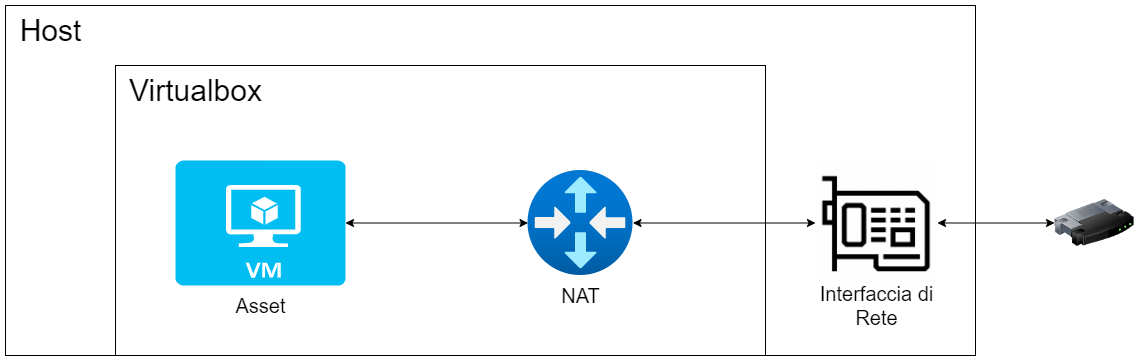
\includegraphics[scale=0.3]{capitoli/figure/schema-rete-nat-solo-asset.png}
    \caption{Infrastruttura di rete}
\end{figure}


\section{Strumenti utilizzati}
Per proseguire con l'analisi dell'asset, è necessario ottenere strumenti appositi che permettono di realizzare scansioni, mapping di vulnerabilità, ecc. Visto che, come già detto in precedenza, l'asset è una \emph{macchina virtuale} che sarà eseguita in un \emph{ambiente di virtualizzazione} e all'interno di una \emph{rete virtuale con NAT}, il modo più semplice per analizzare l'asset è quella di utilizzare una macchina virtuale realizzata apposta per questo scopo. A tal proposito, si è scelto di utilizzare una macchina virtuale molto popolare chiamata \textbf{Kali Linux} (in particolare la versione di riferimento \textbf{2023.1}) che viene distribuito con una suite di strumenti pronti all'uso per effettuare attività di Penetration Testing, Digital Forensics e altre simili. A questo punto, essendo che anche \textbf{Kali Linux} è una macchina virtuale che viene eseguita all'interno di \emph{VirtualBox}, verrà configurata anch'essa in modo tale che si colleghi alla \emph{rete con NAT} creata in precedenza. Otteniamo così il seguente schema:

\begin{figure}[h]
    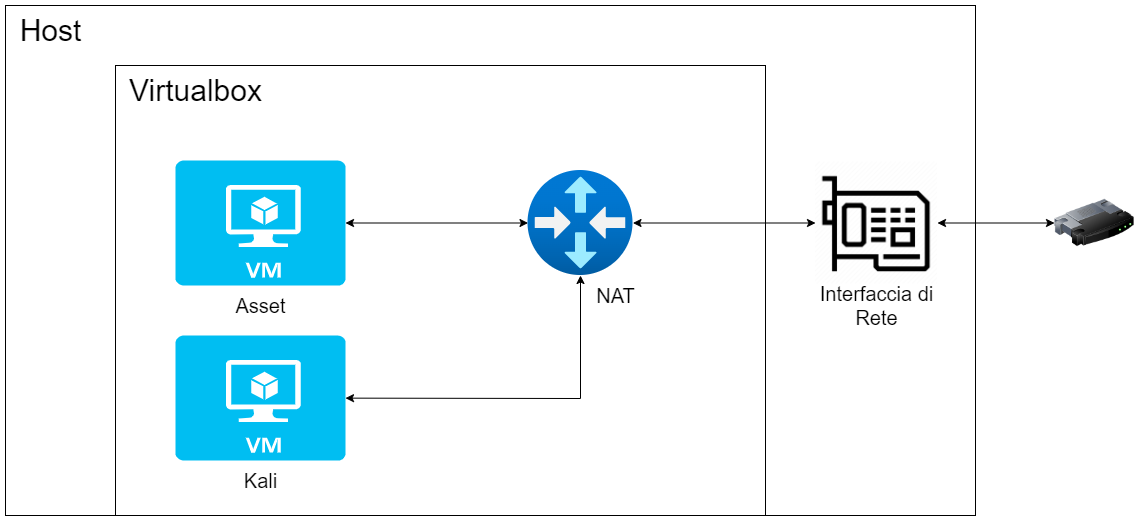
\includegraphics[scale=0.25]{capitoli/figure/schema-rete-nat-kali.png}
    \caption{Infrastruttura di rete con Kali}
\end{figure}
\chapter{Pre-Exploitation}
\markboth{Pre-Exploitation}{}

\section{Target Scoping}
In questa fase bisogna stipulare un accordo tra le parti (responsabile dell'asset e pentester) in modo da definire vincoli, limiti, responsabilità legali in caso di eventuali problemi, accordo di non divulgazione, ecc. Tuttavia, possiamo fare le seguenti osservazioni:

\begin{itemize}
    \item L'asset da analizzare è pubblicamente disponibile e realizzato appositamente per essere analizzato, ossia vulnerabile by-design;
    \item Tutta l'analisi avviene in un ambiente virtualizzato all'interno della macchina in possesso al Penetration Tester;
    \item Lo scopo dell'analisi è puramente didattico, in quanto realizzato in un contesto universitario e, più precisamente, come progetto del corso "Penetration Testing and Ethical Hacking";
    \item Tutti gli strumenti utilizzati e le fonti consultate sono pubblicamente disponibili e accessibili o, in generale, sono accessibili tramite piani gratuiti e quindi senza costi da sostenere.
\end{itemize}

In conclusione, come si può notare dalle precedenti osservazioni, questa fase può essere tranquillamente saltata visto che non ci sono parti con cui prendere accordi e non possono esserci problematiche di tipo legale dal momento che l'ambiente è totalmente simulato.

\section{Information Gathering}
Durante questa fase, l'obiettivo è quello di trovare più informazioni possibili riguardo l'asset scelto e, essendo che l'asset è una macchina virtuale che viene eseguita in un \emph{ambiente virtualizzato} e in una \emph{rete con NAT virtuale} (come illustrato nell'introduzione), si eviteranno fonti e tool che raccolgono informazioni riguardo persone afferenti all'organizzazione dell'asset, indirizzi e-mail, analisi di record DNS, informazioni di routing e così via. A questo punto, l'unica tecnica che ha senso utilizzare (e che è stata effettivamente utilizzata) è \textbf{OSINT} (\emph{Open Source INTelligence}), con cui si cercherà di individuare nomi utente, password, indirizzo IP, ecc. Tutto questo, ovviamente, evitando di consultare fonti dove sono presenti Walktrough e guide per evitare di vanificare il contributo didattico del processo.

Come primo passo, è stata consultata la pagina di Vulnhub sulla quale sono riportate varie informazioni riguardo la macchina virtuale scelta "\textbf{De-ICE S1.140}" e,
all'interno della pagina, sono state trovate le seguenti informazioni:
\begin{itemize}
    \item Informazioni riguardo il \textbf{rilascio}, ovvero autore, data, sorgente e valore hash della macchina. Queste informazioni, tuttavia, non sembrano essere utili per il processo;
    \item Una \textbf{descrizione} molto ad alto livello della macchina. Anche qui non viene rilasciata alcuna informazione utile come servizi esposti dalla macchina o credenziali di accesso alla macchina (anche non privilegiate). Infatti, attualmente, se avviamo la macchina non possiamo fare nulla tramite \emph{interazione diretta} in quanto \textbf{non abbiamo nessuna credenziale di accesso};
    \item Informazioni riguardo la configurazione dell'\textbf{indirizzo di rete}. Questa informazione è molto utile perché ci rivela che la macchina \textbf{non è configurata per lavorare con un indirizzo IP specifico} ma lo ottiene in maniera automatica grazie al servizio \textbf{DHCP}. Questo ci fa subito capire che all'interno della rete con NAT non avremo problemi di indirizzamento ma, sfortunatamente, questo significa che non conosciamo apriori l'indirizzo della macchina (sappiamo solo che sarà all'interno della rete \emph{10.0.2.0/24}) ma dovremo ricavarcelo in maniera indiretta visto che \emph{VirtualBox} non fornisce un metodo diretto di ottenimento degli indirizzi IP e \textbf{non abbiamo accesso alla macchina};
    \item Informazioni riguardo il \textbf{sistema operativo}. Altra informazione molto utile in quanto adesso sappiamo che l'asset è un sistema Linux e questo ci permetterà di risparmiare tempo in fasi avanzate perché possiamo restringere il campo delle scansioni solo a sistemi Linux, escludendo tutti gli altri. Tuttavia, non sappiamo ancora la versione precisa del kernel e quindi dobbiamo ricavarla successivamente;
\end{itemize}

Andando più a fondo nella pagina si può ricavare l'indirizzo del \textbf{sito web del creatore} dell'asset e il \textbf{link di download della macchina} ma, sfortunatamente, entrambi i link \textbf{non sono più attivi}. Consultando il motore di ricerca Google, semplicemente ricercando il nome dell'organizzazione trovato sulla pagina, è possibile risalire al rispettivo account Twitter e si nota che quest'ultimo non è attivo all'incirca dal 2020. Per questa ragione, è sembrato opportuno accedere al servizio \emph{WaybackMachine} offerto da \textbf{Archive.org} per visitare versioni precedenti del sito dell'organizzazione nella speranza di trovare altre informazioni utili. Fortunatamente, grazie a questo servizio è stato possibile accedere ad uno \emph{snapshot} risalente al 2021 dal quale è stato anche possibile effettuare il download della macchina. Ad ogni modo, anche accedendo al sito e, in particolare, alla pagina di download, non sono state trovate informazioni rilevanti come credenziali, porte aperte, schemi di naming, ecc.

\section{Target Discovery}
In questa fase si avvieranno entrambe le macchine e si procederà con la scansione della rete \emph{Corso}, con lo scopo di trovare tutte le macchine attive all'interno della stessa. Ovviamente ci aspettiamo di trovare solo la macchina \textbf{De-ICE S1.140} e la macchina \textbf{Kali} per come abbiamo impostato l'ambiente.

\subsection{Esecuzione di \texttt{ifconfig}}
Prima di cominciare con la scansione effettiva della rete, dobbiamo capire qual è l'indirizzo della macchina \textbf{Kali} in modo da escludere il suo IP da successive scansioni più approfondite. Per ottenere questa informazione ci basta semplicemente lanciare il comando \texttt{ifconfig} e,una volta lanciato questo comando, otteniamo il seguente output:
\begin{figure}[h]
    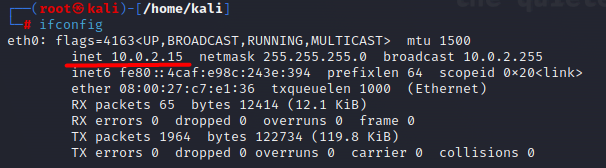
\includegraphics[width=0.8\textwidth]{capitoli/figure/ifconfig-kali.png}
    \centering
    \caption{Esecuzione di \texttt{ifconfig} su Kali}
    \label{fig:ifconfig}
\end{figure}

Come possiamo notare dall'output, l'indirizzo di Kali è \emph{10.0.2.15} e, adesso che lo conosciamo, possiamo cominciare con la scansione della rete.
\subsection{Scansione con \texttt{nmap}}
Il primo strumento utilizzato per la scansione è \texttt{nmap}, un potentissimo strumento di scansione che tornerà molto utile anche nelle successive fasi. In particolare, tra le varie tipologie che offre \texttt{nmap}, permette anche di eseguire una scansione di tipo \textbf{ICMP} (detta \emph{ping scan}) su una determinata sottorete presa in input. Con questa scansione, \texttt{nmap} invierà a tutti gli indirizzi specificati dei pacchetti \emph{ICMP Echo Request} e, se prima dello scadere di un timeout prefissato, riceve da un host un pacchetto \emph{ICMP Echo Reply}, \texttt{nmap} capirà che l’host è attivo e risponde altrimenti marcherà quell’indirizzo come non attivo. Per eseguire una \emph{ping scan} sulla rete \emph{Corso} basta lanciare il seguente comando:

\begin{lstlisting}[language=bash]
    nmap -sP 10.0.2.0/24
\end{lstlisting}

Una volta lanciato questo comando, possiamo osservare il seguente output:
\begin{figure}[h]
    \centering
    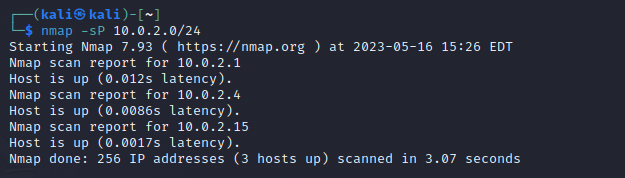
\includegraphics[width=0.8\textwidth]{capitoli/figure/discovery-nmap.png}
    \caption{Risultato della \emph{ping scan} con \texttt{nmap}}
    \label{fig:nmap-ping-scan}
\end{figure}

Il primo dato che dovrebbe risaltare è che il numero degli host attivi sulla rete è 3, e non 2 come in realtà ci si aspettava dalla configurazione realizzata. Tuttavia, come specificato a lezione e approfondito anche nella documentazione di \emph{VirtualBox}, all'interno della rete saranno presenti uno o più host "\emph{fittizi}" che sono necessari allo stesso \emph{VirtualBox} per realizzare la stessa \emph{rete con NAT}. Questi host di solito hanno sempre i primi indirizzi assegnabili, quindi è lecito pensare che l'host con indirizzo \emph{10.0.2.1} sia proprio l'host interno di \emph{VirtualBox} e che l'host con indirizzo \emph{10.0.2.4} sia il nostro asset. Per quanto riguarda \emph{10.0.2.15}, in realtà già lo conosciamo dal comando lanciato prima e sappiamo per certo che è proprio l'indirizzo della macchina \textbf{Kali}.

\subsection{Scansione con \texttt{arp-scan}}
Grazie ad \texttt{nmap} conosciamo gli indirizzi IP degli host attivi all'interno della rete, però in seguito potremmo essere interessati anche agli indirizzi \emph{MAC} corrispondenti. Questo perchè l'infrastruttura di rete è composta da un solo \emph{router virtuale} al quale si collegano tutti gli host (come indicato anche nella Figura \ref{fig:infrastruttura-kali}) e, per questa ragione, è possibile utilizzare anche il protocollo \textbf{ARP} essendo una rete locale. A tal proposito, è stato utilizzato il tool \texttt{arp-scan} che, sfruttando proprio il protocollo \textbf{ARP}, è in grado di ottenere gli indirizzi \emph{MAC} degli host connessi. Per eseguire lo strumento sulla rete, è necessario eseguire il seguente comando:

\begin{lstlisting}[language=bash]
    arp-scan 10.0.2.0/24
\end{lstlisting}

Una volta eseguito questo comando, l'output che viene fornito è il seguente:

\begin{figure}[h]
    \centering
    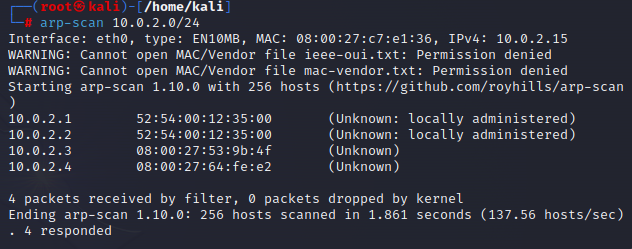
\includegraphics[width=0.8\textwidth]{capitoli/figure/arp-scan.png}
    \caption{Risultato della scansione con \texttt{arp-scan}}
    \label{fig:arp-scan-risultato}
\end{figure}

Anche qui possiamo notare subito un'altra anomalia. Con \texttt{nmap} sono stati rilevati 3 host invece di 2, mentre adesso con \texttt{arp-scan} ne abbiamo rilevati persino 5 (includendo anche la macchina \textbf{Kali} nel conteggio). Osservando con attenzione il risultato, possiamo notare che gli indirizzi \emph{10.0.2.1} e \emph{10.0.2.2} facciano riferimento allo stesso indirizzo MAC (quindi una singola interfaccia con due indirizzi distinti), avvalendo la supposizione precedente che facciano riferimento ad un singolo host interno di \emph{VirtualBox}. A questo punto, se continuiamo a seguire la supposizione che \emph{10.0.2.4} sia l'asset, allora possiamo dire che \emph{10.0.2.3} è un altro host interno di \emph{VirtualBox}. Quindi in realtà gli host attivi non sono 5 come poteva sembrare inzialmente ma sono soltanto 4, e 2 di questi sono host interni di \emph{VirtualBox}.
\subsection{Ulteriore scansione con \texttt{nping}}
A questo punto può sorgere un dubbio, siamo effettivamente sicuri di aver scovato tutti gli host sia "\emph{reali}" che "\emph{fittizi}"? Per essere abbastanza sicuri di averli trovati tutti, evitando così ulteriori sorprese, vale la pena di effettuare un'ulteriore scansione della rete. Per realizzare questa ulteriore scansione è stato utilizzato il tool \texttt{nping}, il quale non fa altro che richiamare il comando \texttt{ping} su tutti gli host forniti in input (quindi ancora una \emph{ping scan}). Per effettuare una scansione con questo tool basta lanciare il seguente comando:

\begin{lstlisting}[language=bash]
    nping -c 1 10.0.2.0/24
\end{lstlisting}

Una volta lanciato il comando otteniamo il seguente output:
\begin{figure}[h]
    \begin{subfigure}{0.5\textwidth}
        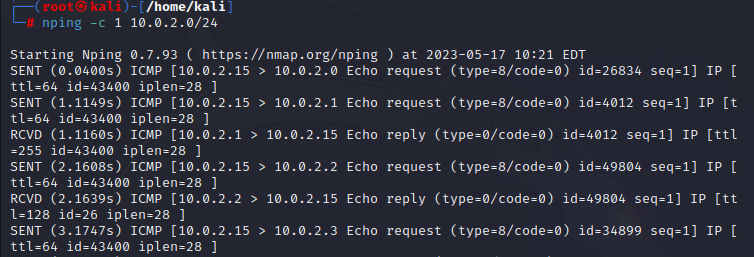
\includegraphics[width=1\textwidth]{capitoli/figure/nping-esecuzione-parziale.png}
        \caption{Esecuzione parziale di \texttt{nping}}
        \label{fig:nping-esecuzione-parziale}
    \end{subfigure}
    \begin{subfigure}{0.5\textwidth}
        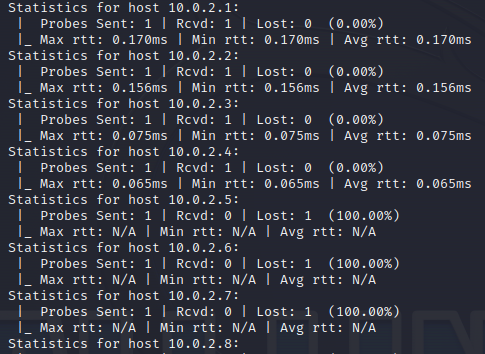
\includegraphics[width=1\textwidth]{capitoli/figure/nping-risultato-parziale.png}
        \caption{Risultato parziale di \texttt{nping}}
        \label{fig:nping-risultato-parziale}
    \end{subfigure}
    \begin{subfigure}{0.9\textwidth}
        \centering
        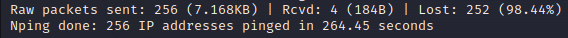
\includegraphics[width=1\textwidth]{capitoli/figure/nping-statistiche.png}
        \caption{Statistiche di \texttt{nping}}
        \label{fig:nping-statistiche}
    \end{subfigure}
    \caption{Output di \texttt{nping}}
\end{figure}

Osservando l'output fornito dal tool \texttt{nping}, sembra che sia conforme con le informazioni ottenute mettendo insieme le precedenti due scansioni. Infatti, possiamo notare dalla Figura \ref{fig:nping-risultato-parziale} che a rispondere al ping sono gli indirizzi \emph{10.0.2.1-4} confermando quindi che sulla rete sono attivi solo 4 host (contando anche la macchina \textbf{Kali}).

\subsection{OS Fingerprinting con \texttt{nmap}}
Con quest'ultima scansione abbiamo terminato di identificare gli host attivi sulla rete e, per questo motivo, possiamo passare al passo successivo. Durante la fase di \emph{Information Gathering} siamo riusciti a stabilire che l'asset è una macchina Linux, ma senza conoscere la versione effettiva del kernel. A tal proposito si può utilizzare ancora una volta il tool \texttt{nmap} che, tramite una tipologia di scansione particolare, è in grado di fare \textbf{OS Fingerprinting} di una determinata macchina presa in input. Per fare ciò, basta eseguire il seguente comando:

\begin{lstlisting}[language=bash]
    nmap -O 10.0.2.4
\end{lstlisting}

Una volta eseguito, l'output ottenuto è il seguente:
\begin{figure}[h]
    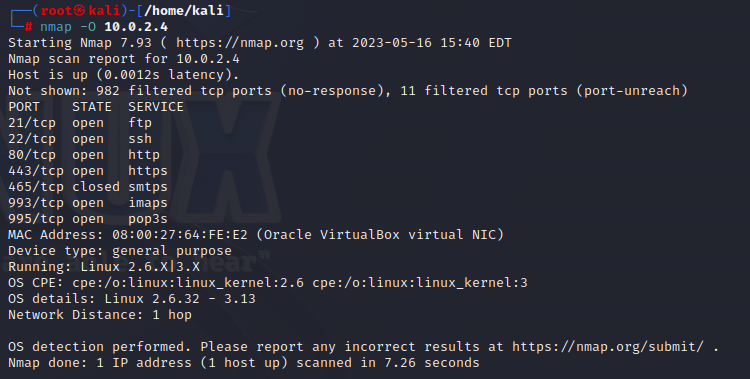
\includegraphics[width=1\textwidth]{capitoli/figure/nmap-os-fingerprint.png}
    \centering
    \caption{Risultato dell'OS Fingerprinting con \texttt{nmap}}
    \label{fig:nmap-os-fingerprint}
\end{figure}

Notiamo che la versione del kernel identificata da \texttt{nmap} risulta essere la \emph{2.6.x/3.x}, in particolare potrebbe trattarsi della versione \emph{2.6.32} o \emph{3.13}. Oltre all'\textbf{OS fingerprint}, possiamo notare che \texttt{nmap} ha eseguito anche una scansione delle porte attive sull'host target. Ovviamente si è limitato solo alle più frequenti (e per questo sarà necessaria una scansione più approfondita nella fase successiva), tuttavia, possiamo notare che ha delle porte aperte che possono essere molto interessanti anche in questo momento. In particolare, le suddette porte sono quelle relative a \textbf{ftp}, \textbf{ssh} e \textbf{http} e, sono particolarmente interessanti poichè si può pensare ad un approfondimento.

\subsection{OS Fingerprint passivo con \texttt{p0f}}
Come accennato in precedenza, grazie a quelle porte aperte si può pensare di fare un'ulteriore scansione ma, questa volta, di tipo passivo. Si può pensare di utilizzare il tool \texttt{p0f}, che si occupa di analizzare il traffico "legittimo" generato da e verso i vari host estrapolando le cosiddette \textbf{Informazioni Caratterizzanti}. Quindi, tutto quello che dobbiamo fare è eseguire il comando \texttt{p0f} e lasciarlo in backround nel mentre che si genera del traffico "legittimo" verso l'asset.

Un primo tentativo che si può fare è quello di generare del traffico \emph{ftp} verso la macchina e, successivamente, controllare se \texttt{p0f} è riuscito ad estrapolare informazioni utili:

\begin{figure}[h]
    \begin{subfigure}{0.5\textwidth}
        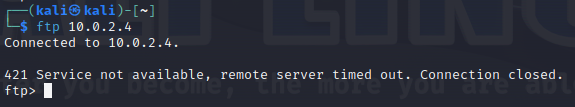
\includegraphics[width=1\textwidth]{capitoli/figure/kali-ftp.png}
        \caption{Generazione di traffico \emph{ftp} legittimo}
        \label{fig:kali-ftp}
    \end{subfigure}
    \begin{subfigure}{0.5\textwidth}
        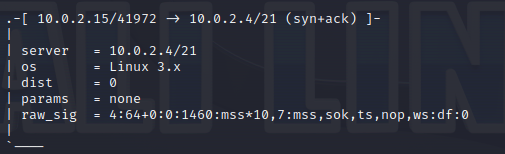
\includegraphics[width=1\textwidth]{capitoli/figure/p0f-ftp.png}
        \caption{Risultato analisi di \texttt{p0f} su traffico \emph{ftp}}
        \label{fig:p0f-ftp}
    \end{subfigure}
\end{figure}

Come si può notare dalla Figura \ref{fig:p0f-ftp}, \texttt{p0f} analizzando il traffico \emph{ftp} è stato in grado di stabilire che il sistema operativo dell'asset ha una versione del kernel \emph{3.x}. Essendo che le tecniche passive non hanno la stessa accuratezza dei metodi attivi (per ovvi motivi), invece di concludere l'analisi con questa informazione è meglio approfondire ulteriormente. A tal proposito, questa volta si è generato del traffico \emph{http} sfruttando il browser \textbf{Mozilla Firefox} installato su \textbf{Kali}. Senza interrompere l'esecuzione di \texttt{p0f}, una volta generato il suddetto traffico è stato ottenuto il seguente output:

\begin{figure}[h]
    \centering
    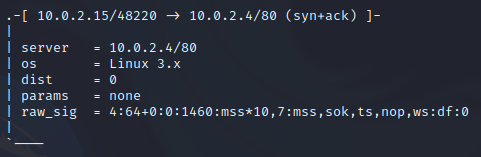
\includegraphics[width=0.7\textwidth]{capitoli/figure/p0f-http.png}
    \caption{Risultato analisi di \texttt{p0f} su traffico \emph{http}}
    \label{fig:p0f-http}
\end{figure}

Consultando anche questo risultato, si può notare che anche qui \texttt{p0f} ha identificato il kernel \emph{3.x}, rendendo più plausibile questa come versione effettiva.

Inoltre, unendo quest'informazione con la scansione attiva realizzata da \texttt{nmap}, è lecito dedurre che molto probabilmente la versione del kernel utilizzata dall'asset sia proprio la versione \emph{3.13}.

\section{Target Enumeration}
\chapter{Exploitation}
\markboth{Exploitation}{}

Adesso che sono state ottenute abbastanza informazioni sulla macchina, si può procedere con la fase di \emph{Exploitation}

\section{Strategie Automatizzate}
Il primo passo eseguito è stato quello di verificare effettivamente quali potevano essere le vulnerabilità sfruttabili consultando tutti i report ottenuti dai tool ed effettivamente le strade più promettenti sono:
\begin{enumerate}
    \item Sfruttamento della vulnerabilità di \textbf{SQL Injection};
    \item Sfruttamento della vulnerabilità di \textbf{mod\_ssl};
    \item Sfruttamento della vulnerabilità di \textbf{ProFTPD};
    \item Sfruttamento della vulnerabilità \textbf{HeartBleed};
    \item Sfruttamento di vulnerabilità di \textbf{phpMyAdmin}
\end{enumerate}

\subsection{Utilizzo di \texttt{sqlmap}}
Per tentare di sfruttare la vulnerabilità di \textbf{SQL Injection} sull'asset si è deciso di utilizzare \texttt{sqlmap}, uno strumento molto potente e in grado di automatizzare il processo di \emph{injection} sulle pagine. Per avviarlo basta eseguire il comando:
\begin{lstlisting}[language=bash]
    sqlmap -u https://10.0.2.4 -a -forms
\end{lstlisting}
dove con \texttt{-u} si specifica l'indirizzo target, con \texttt{-a} si specifica l'intenzione di voler recuperare tutto il possibile (schemi, tabelle, ecc.) e con \texttt{-forms} si specifica l'intenzione di sfruttare i \emph{form} presenti nella pagina.

Eseguendo \texttt{sqlmap} sulle varie pagine dell'asset, i risultati sono i seguenti:
\begin{figure}[h]
    \begin{subfigure}{0.5\textwidth}
        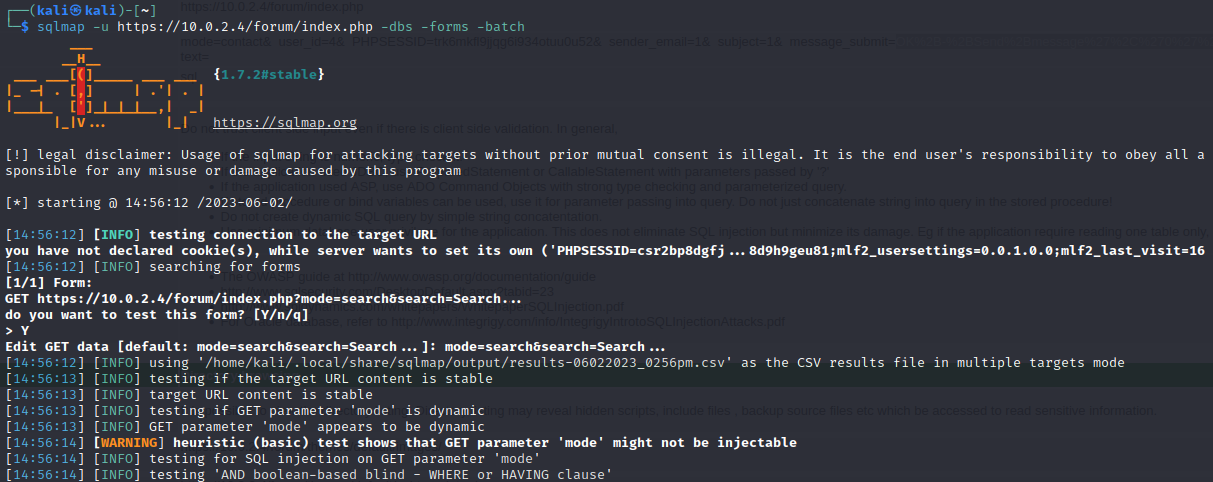
\includegraphics[width=1\textwidth]{capitoli/figure/sqlmap-forum-index-1.png}
        \caption{Prima parte del risultato parziale di \texttt{sqlmap}\\ su \emph{forum/index.php}}
        \label{fig:sqlmap-forum-index-1}
    \end{subfigure}
    \begin{subfigure}{0.5\textwidth}
        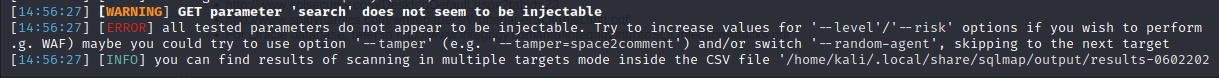
\includegraphics[width=1\textwidth]{capitoli/figure/sqlmap-forum-index-2.png}
        \caption{Seconda parte del risultato parziale di \texttt{sqlmap} su \emph{forum/index.php}}
        \label{fig:sqlmap-forum-index-2}
    \end{subfigure}
    \begin{subfigure}{0.5\textwidth}
        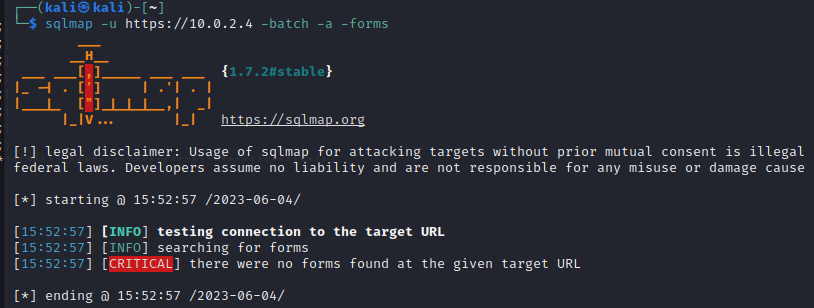
\includegraphics[width=1\textwidth]{capitoli/figure/sqlmap-index.png}
        \caption{Risultato di \texttt{sqlmap} su \emph{index.html}}
        \label{fig:sqlmap-index}
    \end{subfigure}
    \begin{subfigure}{0.5\textwidth}
        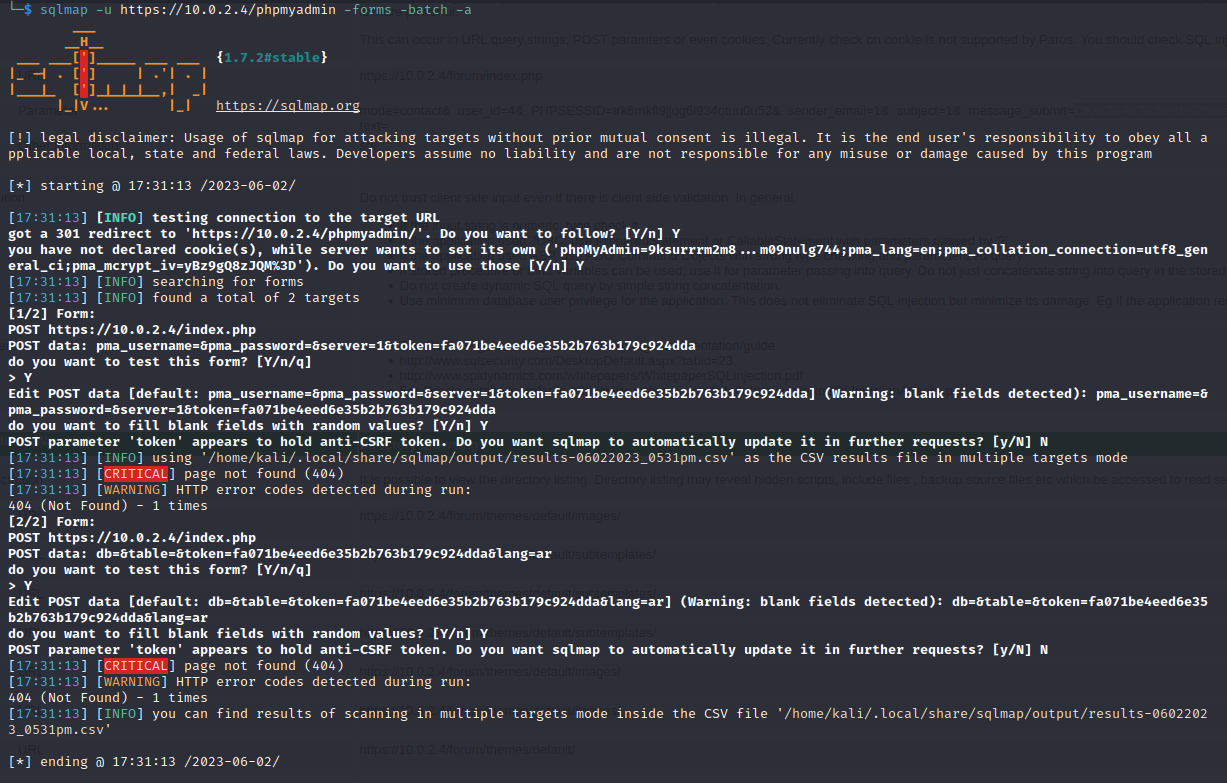
\includegraphics[width=1\textwidth]{capitoli/figure/sqlmap-phpmyadmin.png}
        \caption{Risultato di \texttt{sqlmap} su \emph{phpmyadmin}}
        \label{fig:sqlmap-phpmyadmin}
    \end{subfigure}
    \caption{Risultati ottenuti con \texttt{sqlmap}}
    \label{fig:sqlmap}
\end{figure}

Come si può notare dalle varie esecuzioni di \texttt{sqlmap} si può stabilire che purtroppo lo sfruttamento della \textbf{SQL Injection} non è praticabile e non permette di ottenere ulteriori informazioni. A questo punto, ciò che si può supporre è che il rilevamento effettuato da \texttt{paros} e da \emph{Nessus} non è altro che un falso positivo.

In vista dei risultati ottenuti, quindi, si può scartare questa strategia e procedere con le successive.

\subsection{Utilizzo della suite \emph{Metasploit}}
Il passo successivo è quello di cercare di sfruttare le altre vulnerabilità rilevate riguardo \textbf{mod\_ssl, ProFTPD, HeartBleed} e \textbf{phpMyAdmin}. Utilizzando la suite \emph{Metasploit}, quello che si può fare è cercare degli \emph{exploit} in grado di sfruttare una delle vulnerabilità rilevate dai tool utilizzati per la scansione. Per eseguire la ricerca viene quindi lanciata la console di \emph{Metasploit} con il comando \texttt{msfconsole} e successivamente viene utilizzato il comando \texttt{search}.\\
La prima ricerca effettuata riguarda \textbf{mod\_ssl} e, a quanto rivelato dal report, una versione deprecata di questo strumento potrebbe permettere addirittura l'esecuzione di codice arbitrario da remoto. Tuttavia, effettuando la ricerca non viene trovato nulla a riguardo, come mostrato di seguito:
\begin{figure}[h]
    \centering
    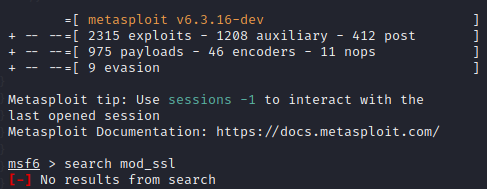
\includegraphics[width=0.5\textwidth]{capitoli/figure/metasploit-mod_ssl.png}
    \caption{Risultato ricerca di \textbf{mod\_ssl}}
    \label{fig:metasploit-modssl}
\end{figure}

Anche effettuando una ricerca sul sito del \emph{MITRE} si scopre che, nonostante questa possibilità, non sono forniti exploit a riguardo.\\
Allora quello che si può fare è continuare la ricerca con \textbf{ProFTPD} e, questa volta, si ottengono dei risultati come mostrato di seguito:
\begin{figure}[h]
    \centering
    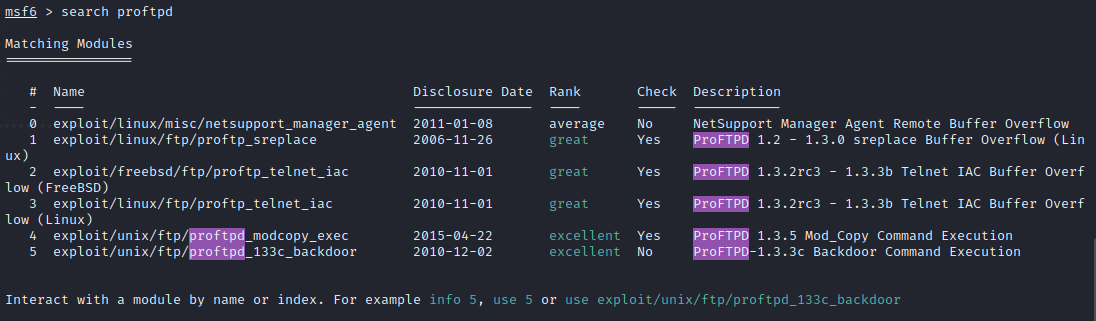
\includegraphics[width=0.6\textwidth]{capitoli/figure/metasploit-proftpd.png}
    \caption{Risultato ricerca di \textbf{ProFTPD}}
    \label{fig:metasploit-proftpd}
\end{figure}

Tenendo presente che la versione di \textbf{ProFTPD} installata è \textbf{1.3.4a}, si nota che solo un exploit potrebbe essere utilizzabile in quanto gli altri sono efficaci solo contro versioni precedenti a quella installata. L'exploit in questione è \textbf{modcopy\_exec} che permette la copia di qualunque file accessibile con i permessi dell'utente che esegue il servizio \textbf{ProFTPD} e anche esecuzione di codice tramite \emph{PHP} \cite{proftpd-mod-copy}.

Selezionando questo exploit e come payload una reverse shell con \emph{netcat} (con le opportune configurazioni),  il risultato è che non si ha successo poichè probabilmente non si hanno i permessi di scrittura sulla cartella target, come mostrato di seugito:
\begin{figure}[h]
    \centering
    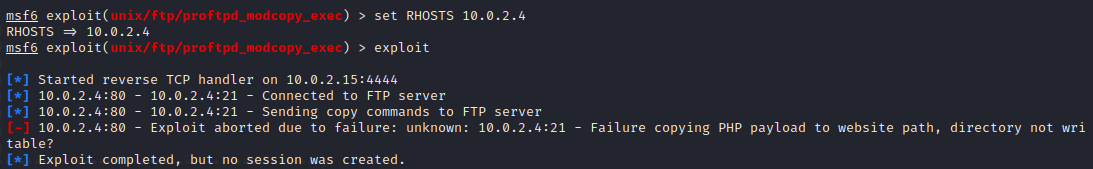
\includegraphics[width=0.5\textwidth]{capitoli/figure/metasploit-proftpd-attack.png}
    \caption{Risultato attacco di \textbf{ProFTPD}}
    \label{fig:metasploit-proftpd-attack}
\end{figure}

Lo stesso risultato è ottenuto anche con tutti gli altri payload, sia di tipo reverse che di tipo bind, rendendo anche questa strada non utilizzabile.\\
Rimossa anche quest'altra strada, un ulteriore tentativo è quello di sfruttare \textbf{HeartBleed}. Come fatto in precedenza, viene effettuata la ricerca di exploit a riguardo e il risultato è il seguente:
\begin{figure}[h]
    \centering
    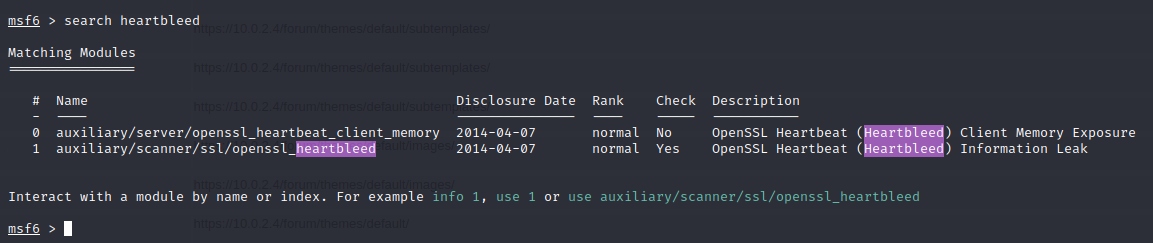
\includegraphics[width=0.7\textwidth]{capitoli/figure/metasploit-heartbleed-list.png}
    \caption{Risultato ricerca di \textbf{HeartBleed}}
    \label{fig:metasploit-heartbleed}
\end{figure}

Non è stato trovato un exploit a riguardo ma un modulo ausiliario, il quale non permette di ottenere una \emph{shell} (quindi il controllo della macchina), ma permette l'ottenimento di altre informazioni che possono tornare molto utili. Se ad esempio si riuscisse a sfruttare questa vulnerabilità, si potrebbero ottenere persino password e chiavi private salvate sul server. Utilizzando lo scanner, tuttavia, il risultato è che ancora una volta non si riesce ad ottenere nulla, come mostrato di seguito:
\begin{figure}[h]
    \centering
    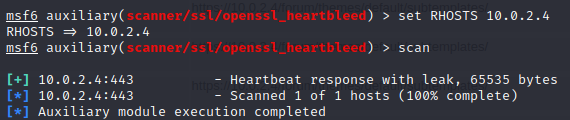
\includegraphics[width=0.6\textwidth]{capitoli/figure/metasploit-heartbleed-scan.png}
    \caption{Risultato attacco con \textbf{HeartBleed}}
    \label{fig:metasploit-heartbleed-attack}
\end{figure}

Infatti l'esecuzione del modulo termina senza ottenere nulla, confermando però la presenza della vulnerabilità \textbf{HeartBleed}.\\
A questo punto non resta che sperare in qualche vulnerabilità di \textbf{phpMyAdmin} (visto che era stata rilevato un falso positivo magari c'è altro) e, effettuando una ricerca, si ottengono i seguenti risultati:
\begin{figure}[h]
    \centering
    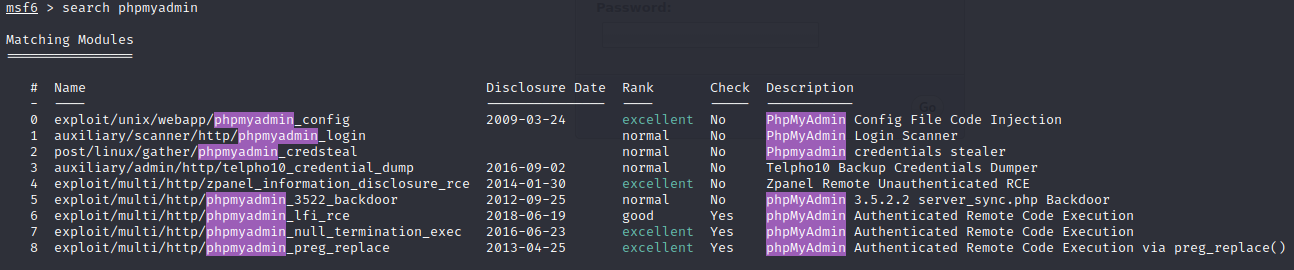
\includegraphics[width=0.7\textwidth]{capitoli/figure/metasploit-phpmyadmin.png}
    \caption{Risultato ricerca di \textbf{phpMyAdmin}}
    \label{fig:metasploit-phpmyadmin}
\end{figure}

Escludendo i moduli \emph{post} (Utilizzabili dopo aver eseguito l'exploitation con successo) e \emph{auxiliary}, gli unici \emph{exploit} interessanti sono gli ultimi 3. Sfortunatamente, dopo l'esecuzione di tutti i payload di tutti e 3 gli exploit, non è stato possibile eseguire l'exploiting della macchina \emph{10.0.2.4}, come mostrato parzialmente di seguito:
\begin{figure}[h]
    \centering
    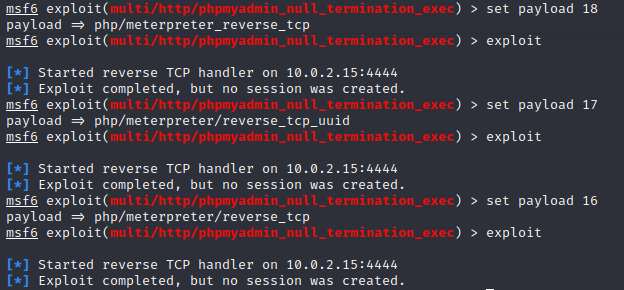
\includegraphics[width=0.7\textwidth]{capitoli/figure/metasploit-phpmyadmin-attack.png}
    \caption{Risultato parziale dell'attacco a \textbf{phpMyAdmin}}
    \label{fig:metasploit-phpmyadmin-attack}
\end{figure}

Purtroppo, dopo quest'ultimo fallimento, non sembrano esserci altre vie percorribili basandosi sulle informazioni acquisite in precedenza.

\subsection{Utilizzo della GUI \emph{Armitage}}
Un ultimo tentativo che è possibile realizzare è quello di utlizzare \emph{Armitage}, una GUI per la suite \emph{Metasploit}. Il motivo è per utilizzare una funzione offerta chiamata \textbf{Hail Mary}, che si occupa di effettuare il bruteforce di tutti gli exploit e payload compatibili su una macchina target nella speranza di instaurare almeno una \emph{sessione}. Per utilizzare la funzione precedentemente citata, bisogna effettuare di nuovo le fasi target discovery ed enumeration all'interno di \emph{Armitage} e, una volta finite, basta utilizzare l'opzione \emph{find attacks} per filtrare gli exploit che sono compatibili con la macchina target. Il risultato ottenuto fino a questo momento è il seguente:
\begin{figure}[h]
    \centering
    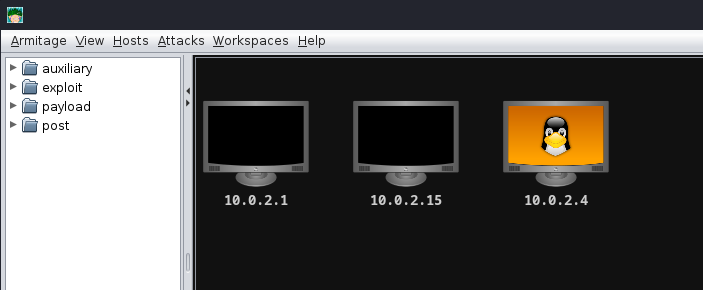
\includegraphics[width=0.7\textwidth]{capitoli/figure/armitage.png}
    \caption{Output di \emph{Armitage} dopo le scansioni}
    \label{fig:armitage}
\end{figure}

A questo punto è possibile lanciare la funzione \emph{Hail Mary} e, dopo aver atteso che tutti gli exploit siano stati lanciati, si può osservare che anche con questa strategia \emph{estrema} non è stato possibile avere accesso alla macchina. Un report con gli exploit lanciati da questa funzione è consultabile nella cartella \emph{Report} con il nome \textbf{armitage-hailmary.log}.

\subsection{Fallimento delle strategie automatizzate}
Nonostante i report fossero promettenti inizialmente, visto che sono state trovate trovate vulnerabilità interessanti, l'utilizzo di strumenti automatici per l'exploitation non ha mostrato i risultati sperati e si è rivelato un completo fallimento. Una possibile ragione per cui questo è accaduto può essere il fatto che l'asset da attaccare in realtà è una macchina che non è stata pensata per un \emph{Penetration Testing} ma bensì per una \emph{sfida CTF}. Questo significa, quindi, che la macchina non è stata realizzata utilizzando servizi vulnerabili (sarebbe stata facilitata la risoluzione della \emph{sfida CTF}) ma utilizzando servizi "aggiornati" (ovviamente in riferimento alle versioni dell'anno di rilascio) che non presentano vulnerabilità tali da fornire accesso completo o parziale alla macchina e navigazione libera del file system della macchina ma che permettono ugualmente di effettuare la \emph{CTF}. In base a questa osservazione non ci sono quindi altri modi per avere accesso alla macchina se non quello di risolvere la sfida interrogando manualmente la macchina ed estrapolando nuove informazioni fornite dai servizi offerti.

\section{Strategie manuali}
La decisione presa, a questo punto, è quella di procedere con l'analisi manuale dell'asset.
\subsection{Visita del server web}
La prima interazione eseguita è semplicemente quella di interrogare l'asset in maniera legittima sulla porta 80. L'output che si può osservare è il seguente:
\begin{figure}[h]
    \centering
    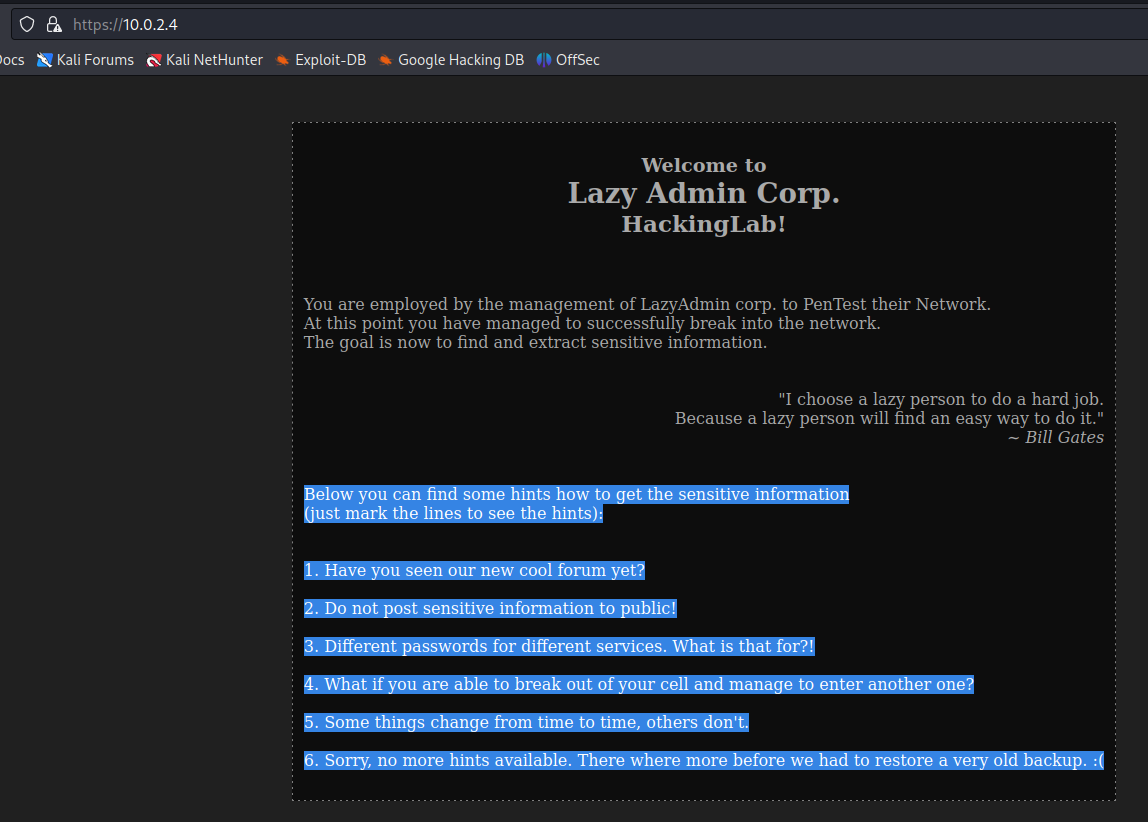
\includegraphics[width=0.5\textwidth]{capitoli/figure/web-index.png}
    \caption{Welcome page dell'asset}
    \label{fig:web-index}
\end{figure}

Evidenziando il testo (come indicato nel suggerimento) si possono ricavare informazioni molto utili:
\begin{itemize}
    \item Viene indicata la presenza di un \textbf{forum}, che già era noto dall'output di \texttt{dirb} e \texttt{nikto};
    \item Viene specificato che non dovrebbero essere \emph{postate} informazioni sensibili in pubblico, quasi come se qualcuno avesse postato delle credenziali (verosimilmente) sul forum;
    \item La presenza di un \textbf{backup} molto vecchio che è stato ripristinato;
\end{itemize}

Non sembrano esserci ulteriori informazioni utili sulla pagina, quindi si può procedere.

\subsection{Accesso al servizio \emph{FTP}}
Prima di continuare con la visita delle pagine web, dalle scansioni precedenti è stato rilevato che il servizio \textbf{ProFTPD} ammette login \emph{anonimi}, per cui vale la pena di tentare una connessione e capire se ci sono file utili a cui si hanno accesso. Eseguendo una connessione anonima, il risultato è il seguente:
\begin{figure}[h]
    \centering
    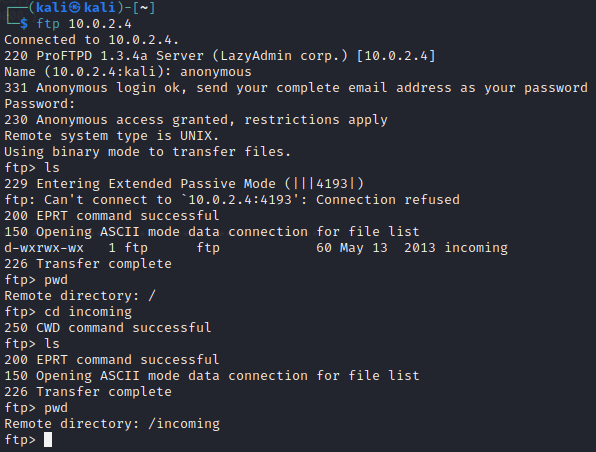
\includegraphics[width=0.5\textwidth]{capitoli/figure/ftp-anon.png}
    \caption{Login anonimo sul servizio \emph{FTP}}
    \label{fig:ftp-anon}
\end{figure}

Quello che si nota è che purtroppo si ha accesso solo ad una cartella di nome \textbf{incoming} che è vuota. Molto probabilmente questo è dovuto al fatto che con il login anonimo non si hanno i permessi per visualizzare il contenuto della suddetta cartella. Quindi al momento non è possibile accedere a nessun file presente sull'asset, però, il nome della cartella ricorda il nome di una \emph{casella di posta} (in italiano \emph{In arrivo}) e questa informazione è coerente anche con la presenza della pagina \textbf{webmail} rilevata da \texttt{nikto}. Ad ogni modo, si può tornare con la consultazione delle pagine web.

\subsection{Analisi della pagina forum}
In base alle informazioni prese dalla \emph{welcome page} dell'asset, il prossimo passo è la visita della pagina \emph{forum}. La pagina si presenta come mostrato di seguito:
\begin{figure}[h]
    \centering
    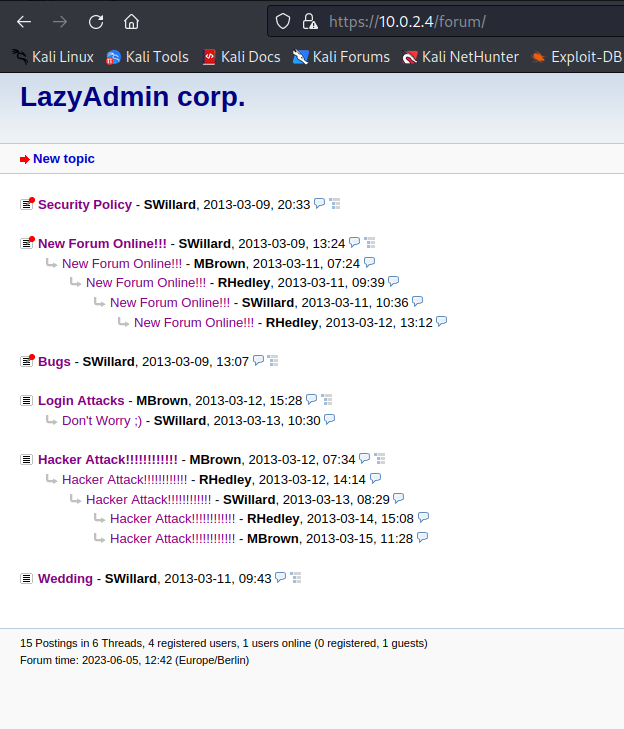
\includegraphics[width=0.4\textwidth]{capitoli/figure/forum.png}
    \caption{Pagina web del \emph{forum}}
    \label{fig:forum}
\end{figure}

Visitando le varie discussioni presenti, salta all'occhio una discussione con il nome \textbf{Login Attacks}, il cui contenuto parziale è mostrato di seguito:
\begin{figure}[h]
    \centering
    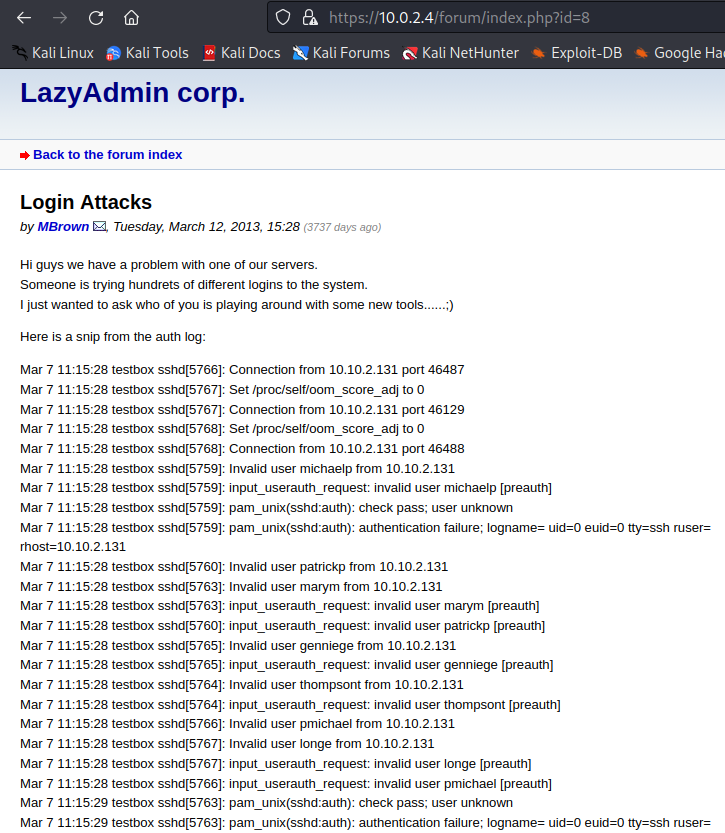
\includegraphics[width=0.4\textwidth]{capitoli/figure/forum-ssh-log.png}
    \caption{Contenuto parziale della discussione \textbf{Login Attacks}}
    \label{fig:forum-ssh-log}
\end{figure}

Leggendo la discussione, si nota che il contenuto riguarda un log di accessi falliti tramite \emph{SSH}. Copiando l'intero contenuto su un file di testo, è stato utilizzato il comando \texttt{grep} per estrarre i nomi utente utilizzati nell'attacco in maniera più agevole e veloce. I nomi utente rilevati sono i seguenti:
\begin{figure}[h]
    \centering
    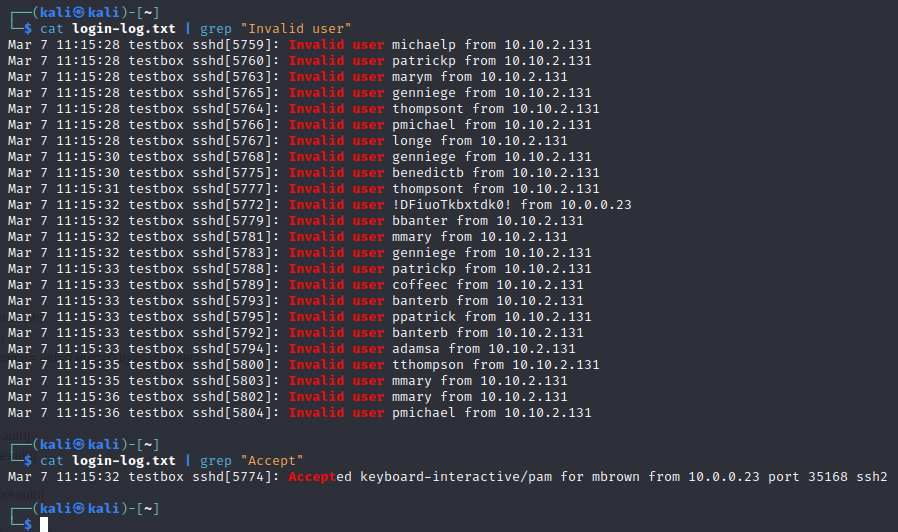
\includegraphics[width=0.4\textwidth]{capitoli/figure/ssh-log-grep.png}
    \caption{Nomi utente estratti con \texttt{grep}}
    \label{fig:ssh-log-grep}
\end{figure}

Dai risultati si possono notare 2 aspetti particolari:
\begin{itemize}
    \item C'è un unico login riuscito con il nome utente \textbf{mbrown}
    \item È presente il nome utente \textbf{!DFiuoTkbxtdk0!} che non sembra avere esattamente l'aspetto di un nome utente ma, piuttosto, sembra essere una \emph{password}.
\end{itemize}

\subsection{Compromissione di un utente del forum}
Notando che il nome dell'utente che ha postato la discussione è proprio \textbf{MBrown}, presente anche nei log trovati, è lecito supporre che l'utente \textbf{mbrown} presente nell'attacco sia lo stesso del forum. Per questo motivo, per la stranezza di uno dei nomi utente (evidenziato in precedenza) e per la tendenza delle persone ad usare la stessa password per servizi diversi, vale la pena tentare un attacco a dizionario sul login del forum con tutte le combinazioni dei nomi utente. Dopo alcuni tentativi falliti, una combinazione funzionante è stata:
\begin{itemize}
    \item \textbf{Nome Utente}: mbrown
    \item \textbf{Password}: !DFiuoTkbxtdk0!
\end{itemize}
Questo ha confermato i sospetti sulla stranezza del nome utente, e il login con le credenziali ci ha dato accesso alla pagina personale dell'utente \textbf{mbrown}, che ha il seguente aspetto:
\begin{figure}[h]
    \centering
    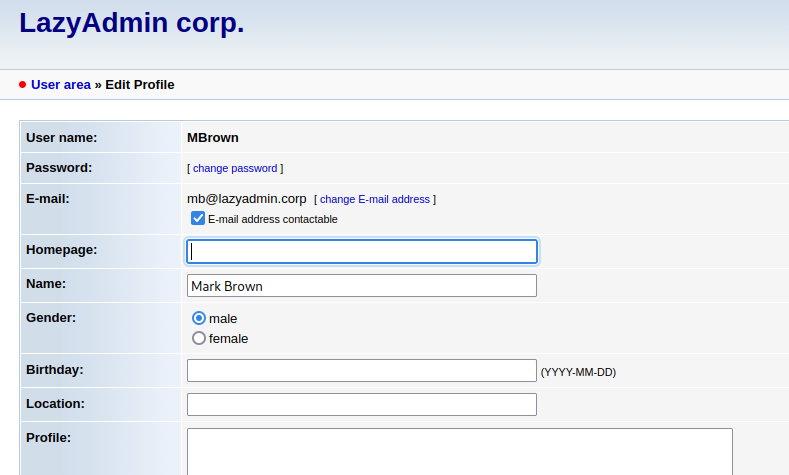
\includegraphics[width=0.4\textwidth]{capitoli/figure/forum-accesso.png}
    \caption{Pagina personale dell'utente \textbf{mbrown}}
    \label{fig:forum-accesso}
\end{figure}

L'unica informazione che sembra essere utile all'interno della pagina è la mail dell'utente compromesso, che è \textbf{mb@lazyadmin.corp}. A questo punto, ricordandoci anche della presenza di una pagina \emph{webmail}, vale la pena tentare l'accesso sulla \emph{webmail} specificando la mail appena trovata e la password appena utilizzata, sfruttando ancora la tendenza delle persone ad utilizzare la stessa password per servizi diversi.

Inaspettatamente, il tentativo ha successo e viene mostrata la pagina seguente:
\begin{figure}[h]
    \centering
    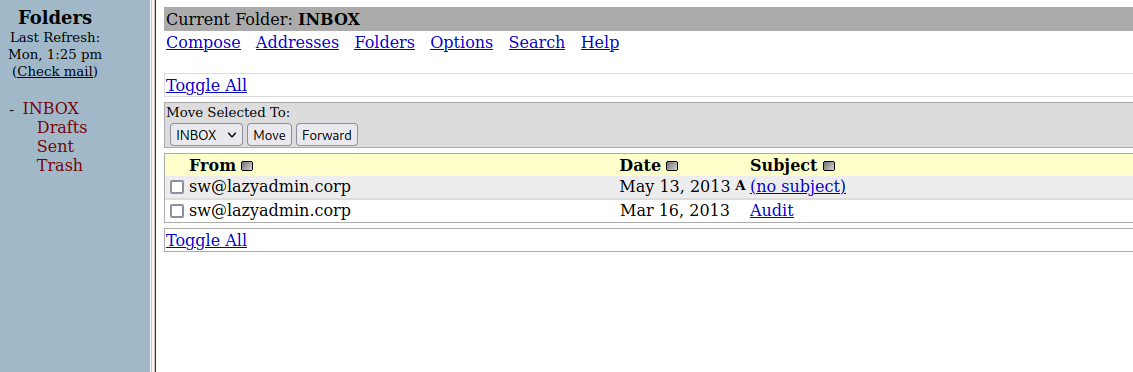
\includegraphics[width=0.5\textwidth]{capitoli/figure/mail-accesso.png}
    \caption{Pagina \emph{webmail} dell'utente \textbf{mbrown}}
    \label{fig:mail-accesso}
\end{figure}

Sono presenti due mail e il contenuto di una delle due è il seguente:
\begin{figure}[h]
    \centering
    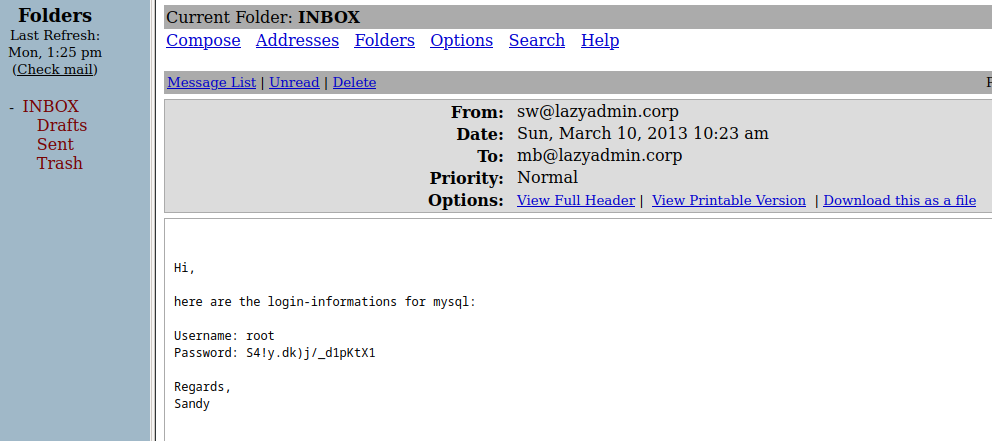
\includegraphics[width=0.5\textwidth]{capitoli/figure/mail-password.png}
    \caption{Una delle mail dell'utente \textbf{mbrown}}
    \label{fig:mail-password}
\end{figure}

È stata comunicata la password dell'utente \textbf{root} del servizio \textbf{phpMyAdmin}.

\subsection{Compromissione di \textbf{phpMyAdmin}}
Ovviamente, andando sulla pagina \emph{phpmyadmin} e immettendo le credenziali ottenute dalla mail, il risultato è che si riesce ad accedere come utente \textbf{root} e viene visualizzata la pagina mostrata di seguito:
\begin{figure}[h]
    \centering
    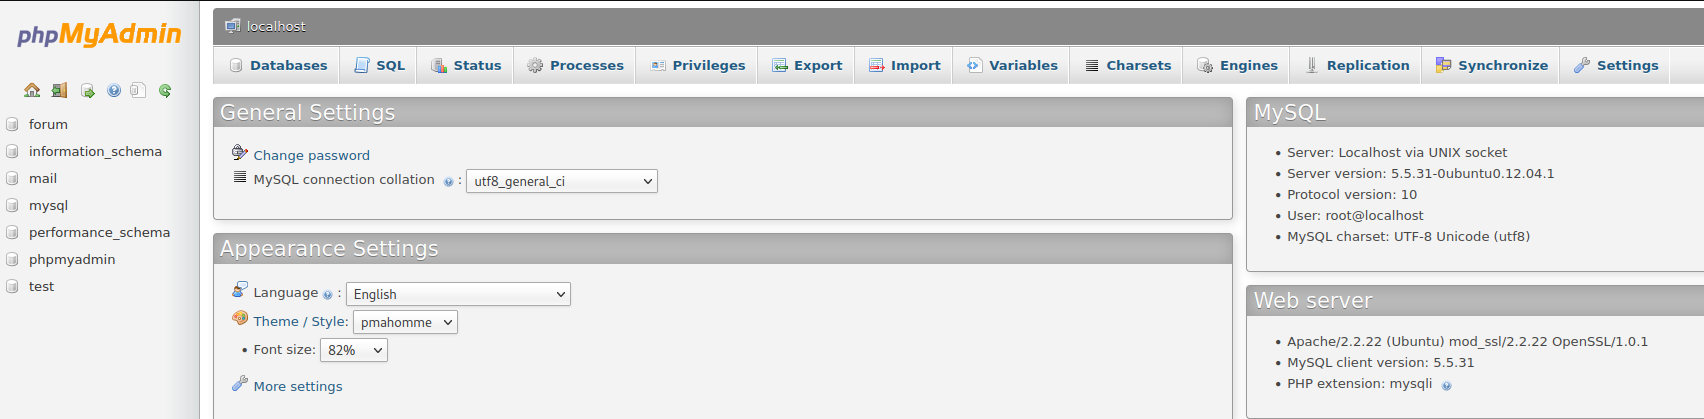
\includegraphics[width=0.5\textwidth]{capitoli/figure/phpmyadmin.png}
    \caption{Pagina dell'utente \textbf{root} su \emph{phpmyadmin}}
    \label{fig:phpmyadmin}
\end{figure}

Esplorando un po' i database presenti, sono di particolare interesse i database \textbf{forum} e \textbf{mail} dove tra tutte le tabelle presenti ci sono delle tabelle una chiamata \emph{ mlf2\_userdata} e l'altra \emph{mailbox}. Aprendo queste tabelle si possono recuperare gli hash delle password di alcuni degli utenti.

\subsection{Cracking degli hash ottenuti}
Questi hash recuperati sono stati salvati in un file e dati in pasto ad un tool di \emph{Offline Password cracking} chiamato \texttt{john} che, dopo un po' di tentativi con wordlist diverse, non è riuscito ad ottenere le corrispondenti password. Dal momento che l'utilizzo di altri strumenti con le stesse \emph{wordlist} si suppone che diano lo stesso risultato, si è tentato di sfruttare risorse sul web nella speranza che qualcuno abbia effettuato il cracking degli hash ottenuti. La ricerca è iniziata su \emph{crackstation.com} dove sfortunatamente non è stato trovato nulla e, successivamente, con una semplice ricerca su \emph{google} degli hash, è stato trovato il sito \emph{md5.gromweb.com} dove è stato possibile reperire 3 password. Il risultato ottenuto è mostrato di seguito:
\begin{figure}[h]
    \centering
    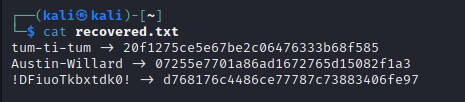
\includegraphics[width=0.7\textwidth]{capitoli/figure/hash-recovered.png}
    \caption{Le tre password recuperate}
    \label{fig:hash-recovered}
\end{figure}

Le password sono rispettivamente di \textbf{Richard Hedley} e \textbf{Sandy Willard}, due utenti che sono iscritti sul forum con i nomi \textbf{RHedley} e \textbf{SWillard}.

\subsection{Tentativo di accesso}
Ora che sono state recuperate le password di tre utenti, quello che si può fare è tentare di accedere al sistema con uno di questi, tuttavia ancora non si conoscono i nomi utenti del sistema ma solo quelli del forum. Ricordando per un attimo il log trovato sul forum, si può notare che un tentativo di accesso riuscito è stato realizzato con il nome utente \textbf{mbrown}, l'utente di cui è stato violato l'account del forum. Un tentativo che si può fare è utilizzare questo nome utente per provare ad accedere al sistema tramite \emph{SSH} o \emph{FTP} utilizzando la password che è stata scoperta. Tuttavia il risultato è mostrato nella Figura \ref{fig:ssh-ftp-incorrect}
\begin{figure}[h]
    \centering
    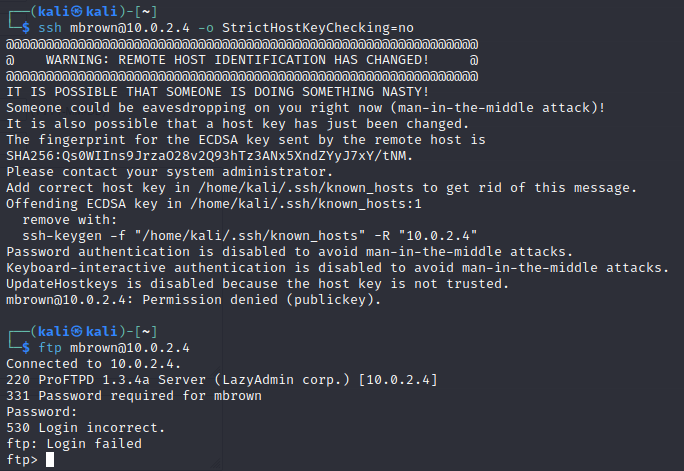
\includegraphics[width=0.6\textwidth]{capitoli/figure/ssh-ftp-incorrect.png}
    \caption{Tentativi di login con l'utente \textbf{mbrown}}
    \label{fig:ssh-ftp-incorrect}
\end{figure}

Per quanto concerne \emph{SSH} essendo che la macchina \textbf{Kali} non è un host riconosciuto, l'autenticazione tramite password è disabilitata e viene richiesto un file di autenticazione (una chiave con cui autenticare la chiave pubblica), quindi non è possibile al momento utilizzare \emph{SSH} (verosimilmente anche con gli altri utenti).\\
Invece, per quanto riguarda \emph{FTP}, a quanto sembra la password non è la stessa che è stata utilizzata in precedenza quindi non si può effettuare il login con l'utente \textbf{mbrown}.

\subsection{Accesso al servizio FTP come nuovo utente}
Essendo che l'utente \textbf{Mark Brown} ha come nome utente sul forum \textbf{MBrown} e come nome utente di sistema \textbf{mbrown}, molto probabilmente questo schema è mantenuto anche dagli altri utenti del sistema. Seguendo questo presupposto, viene effettuato un tentativo con l'utente \textbf{Richard Hedley} e, con un po' di fortuna, il risultato è il seguente:
\begin{figure}[h]
    \centering
    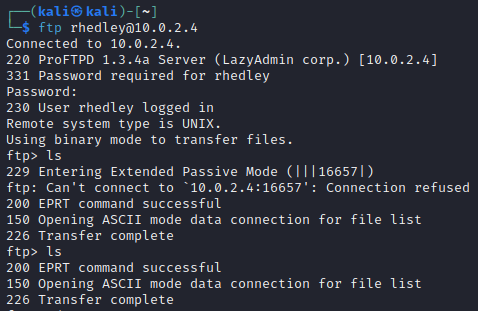
\includegraphics[width=0.5\textwidth]{capitoli/figure/ftp-rhedley.png}
    \caption{Accesso \emph{FTP} con l'utente \textbf{rhedley}}
    \label{fig:ftp-rhedley}
\end{figure}

È stato eseguito il login con successo e, a questo punto, quello che si può fare è esplorare un po' i file accessibili dall'utente. Quello che si può notare è che l'utente utilizzato ha accesso alla cartella dell'utente \textbf{mbrown} e andando nella cartella \textbf{.ssh} (dove \emph{OpenSSH} salva i file relativi alle chiavi) si trova un file \textbf{downloadkey} al quale l'utente può accedere, come mostrato di seguito:
\begin{figure}[h]
    \begin{subfigure}{0.6\textwidth}
        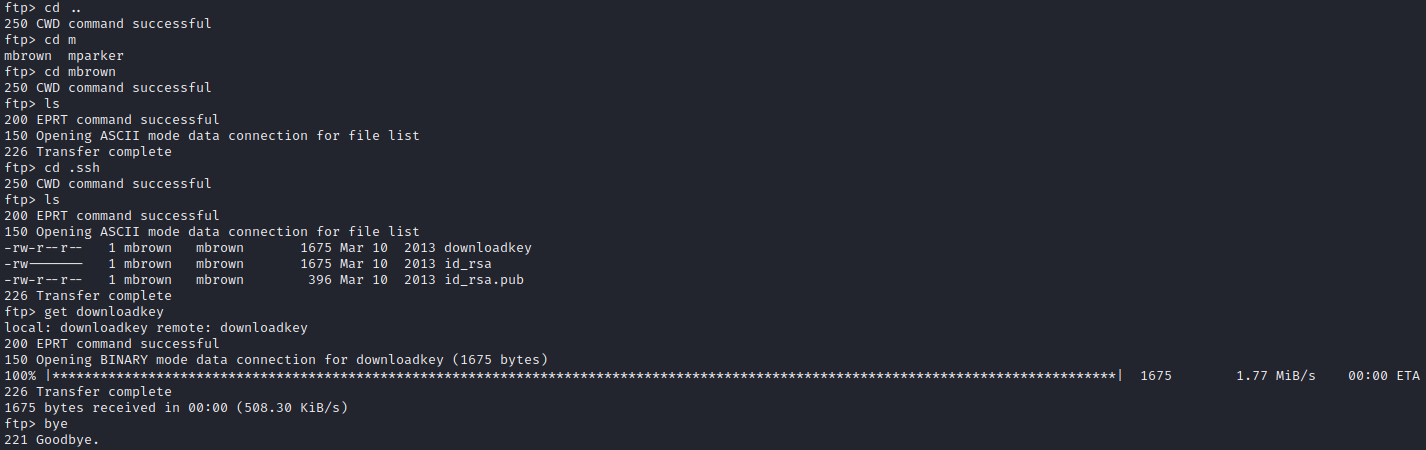
\includegraphics[width=1\textwidth]{capitoli/figure/ftp-rhedley-private-key.png}
        \caption{Download della chiave di \textbf{mbrown}}
        \label{fig:ftp-rhedley-private}
    \end{subfigure}
    \begin{subfigure}{0.4\textwidth}
        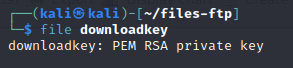
\includegraphics[width=1\textwidth]{capitoli/figure/file-downloadkey.png}
        \caption{Verifica della tipologia di chiave di \textbf{mbrown}}
        \label{fig:file-downloadkey}
    \end{subfigure}
    \caption{Ottenimento della chiave privata di \textbf{mbrown}}
    \label{fig:mbrown-private-key}
\end{figure}

Una volta ottenuto il file \textbf{downloadkey}, utilizzando il comando \texttt{file} è stato possibile accertarsi che il file sia effettivamente una \textbf{chiave privata}.

\subsection{Ottenimento di una shell}
Dal momento che grazie all'utente \textbf{rhedley} è stato possibile recuperare la chiave privata dell'utente \textbf{mbrown}, adesso è possibile effettuare l'accesso all'asset tramite \emph{SSH} utilizzando il seguente comando:
\begin{lstlisting}[language=bash]
    ssh -i downloadkey mbrown@10.0.2.4 -o StrictHostKeyChecking=no
\end{lstlisting}

È stato necessario aggiungere anche il parametro \texttt{StrictHostKeyChecking=no} poichè, dal momento che ad ogni riavvio l'asset rigenera la propria chiave \emph{SSH}, \emph{OpenSSH} solleva un warning e chiude la connessione in via preventiva per evitare attacchi \textbf{Man-In-The-Middle} (visto che la chiave pubblica precedentemente salvata è cambiata) e, per evitare la chiusura, si aggiunge il parametro per ignorare quest'allerta.\\
In seguito all'esecuzione del comando, il risultato è il seguente:
\begin{figure}[h]
    \centering
    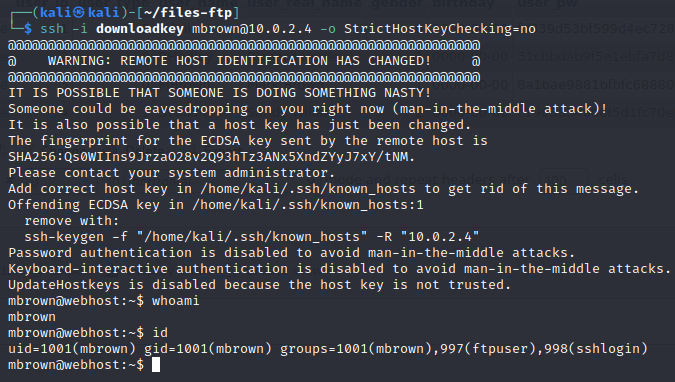
\includegraphics[width=0.5\textwidth]{capitoli/figure/ssh-mbrown.png}
    \caption{Ottenimento della shell come utente \textbf{mbrown}}
    \label{fig:ssh-mbrown}
\end{figure}

Adesso che è stata ottenuta una shell sull'asset, la fase di \emph{Exploitation} può dirsi conclusa con successo.
\chapter{Post-Exploitation}
\markboth{Post-Exploitation}{}

\section{Privilege Escalation}
Ora che è stato ottenuto l'accesso al sistema, il prossimo passo è quello di ottenere quanti più privilegi possibile.

\subsection{Fallimento delle strategie automatizzate}

\subsection{Privilege Escalation orizzontale}

\subsection{Scoperta di un backup}

\subsection{Decifratura del backup}

\subsection{Cracking delle password trovate all'interno del backup}

\subsection{Privilege Escalation Verticale}

\section{Maintaining Access}

\subsection{Crezione della backdoor}

\subsection{Trasferimento della backdoor sull'asset}

\subsection{Abilitazione della backdoor}

\subsection{Impossibilità di testing della backdoor}

%\part{Impatto ambientale}

\backmatter
%*******************************************************
% Bibliografia
%*******************************************************
\cleardoublepage
\phantomsection
\addcontentsline{toc}{chapter}{\bibname}
\nocite{*}
\bibliographystyle{classic}
\bibliography{bibliografia}
%


\end{document}
